\documentclass[landscape]{article}
\usepackage{{./../static/style}}

\pdfinfo{
  /Title (PyAnsys Cheatsheets)
  /Creator (TeX)
  /Producer (pdfTeX 1.40.0)
  /Author (Ansys Inc.,)
  /Subject (PyMotorCAD)
  /Keywords (PyMotorCAD)}

% -----------------------------------------------------------------------

\begin{document}
\raggedright
\footnotesize
\begin{center}
     \Huge{\textbf{PyMotorCAD-API Cheatsheet}} 
\end{center}
\begin{center}
	\small{\textbf{based on version:0.1 (stable)}} 
\end{center}
\AddToShipoutPicture*
  {\put(670,577.5){
\includegraphics[height = 1.2cm]{ansys.png}}}
\AddToShipoutPictureBG*{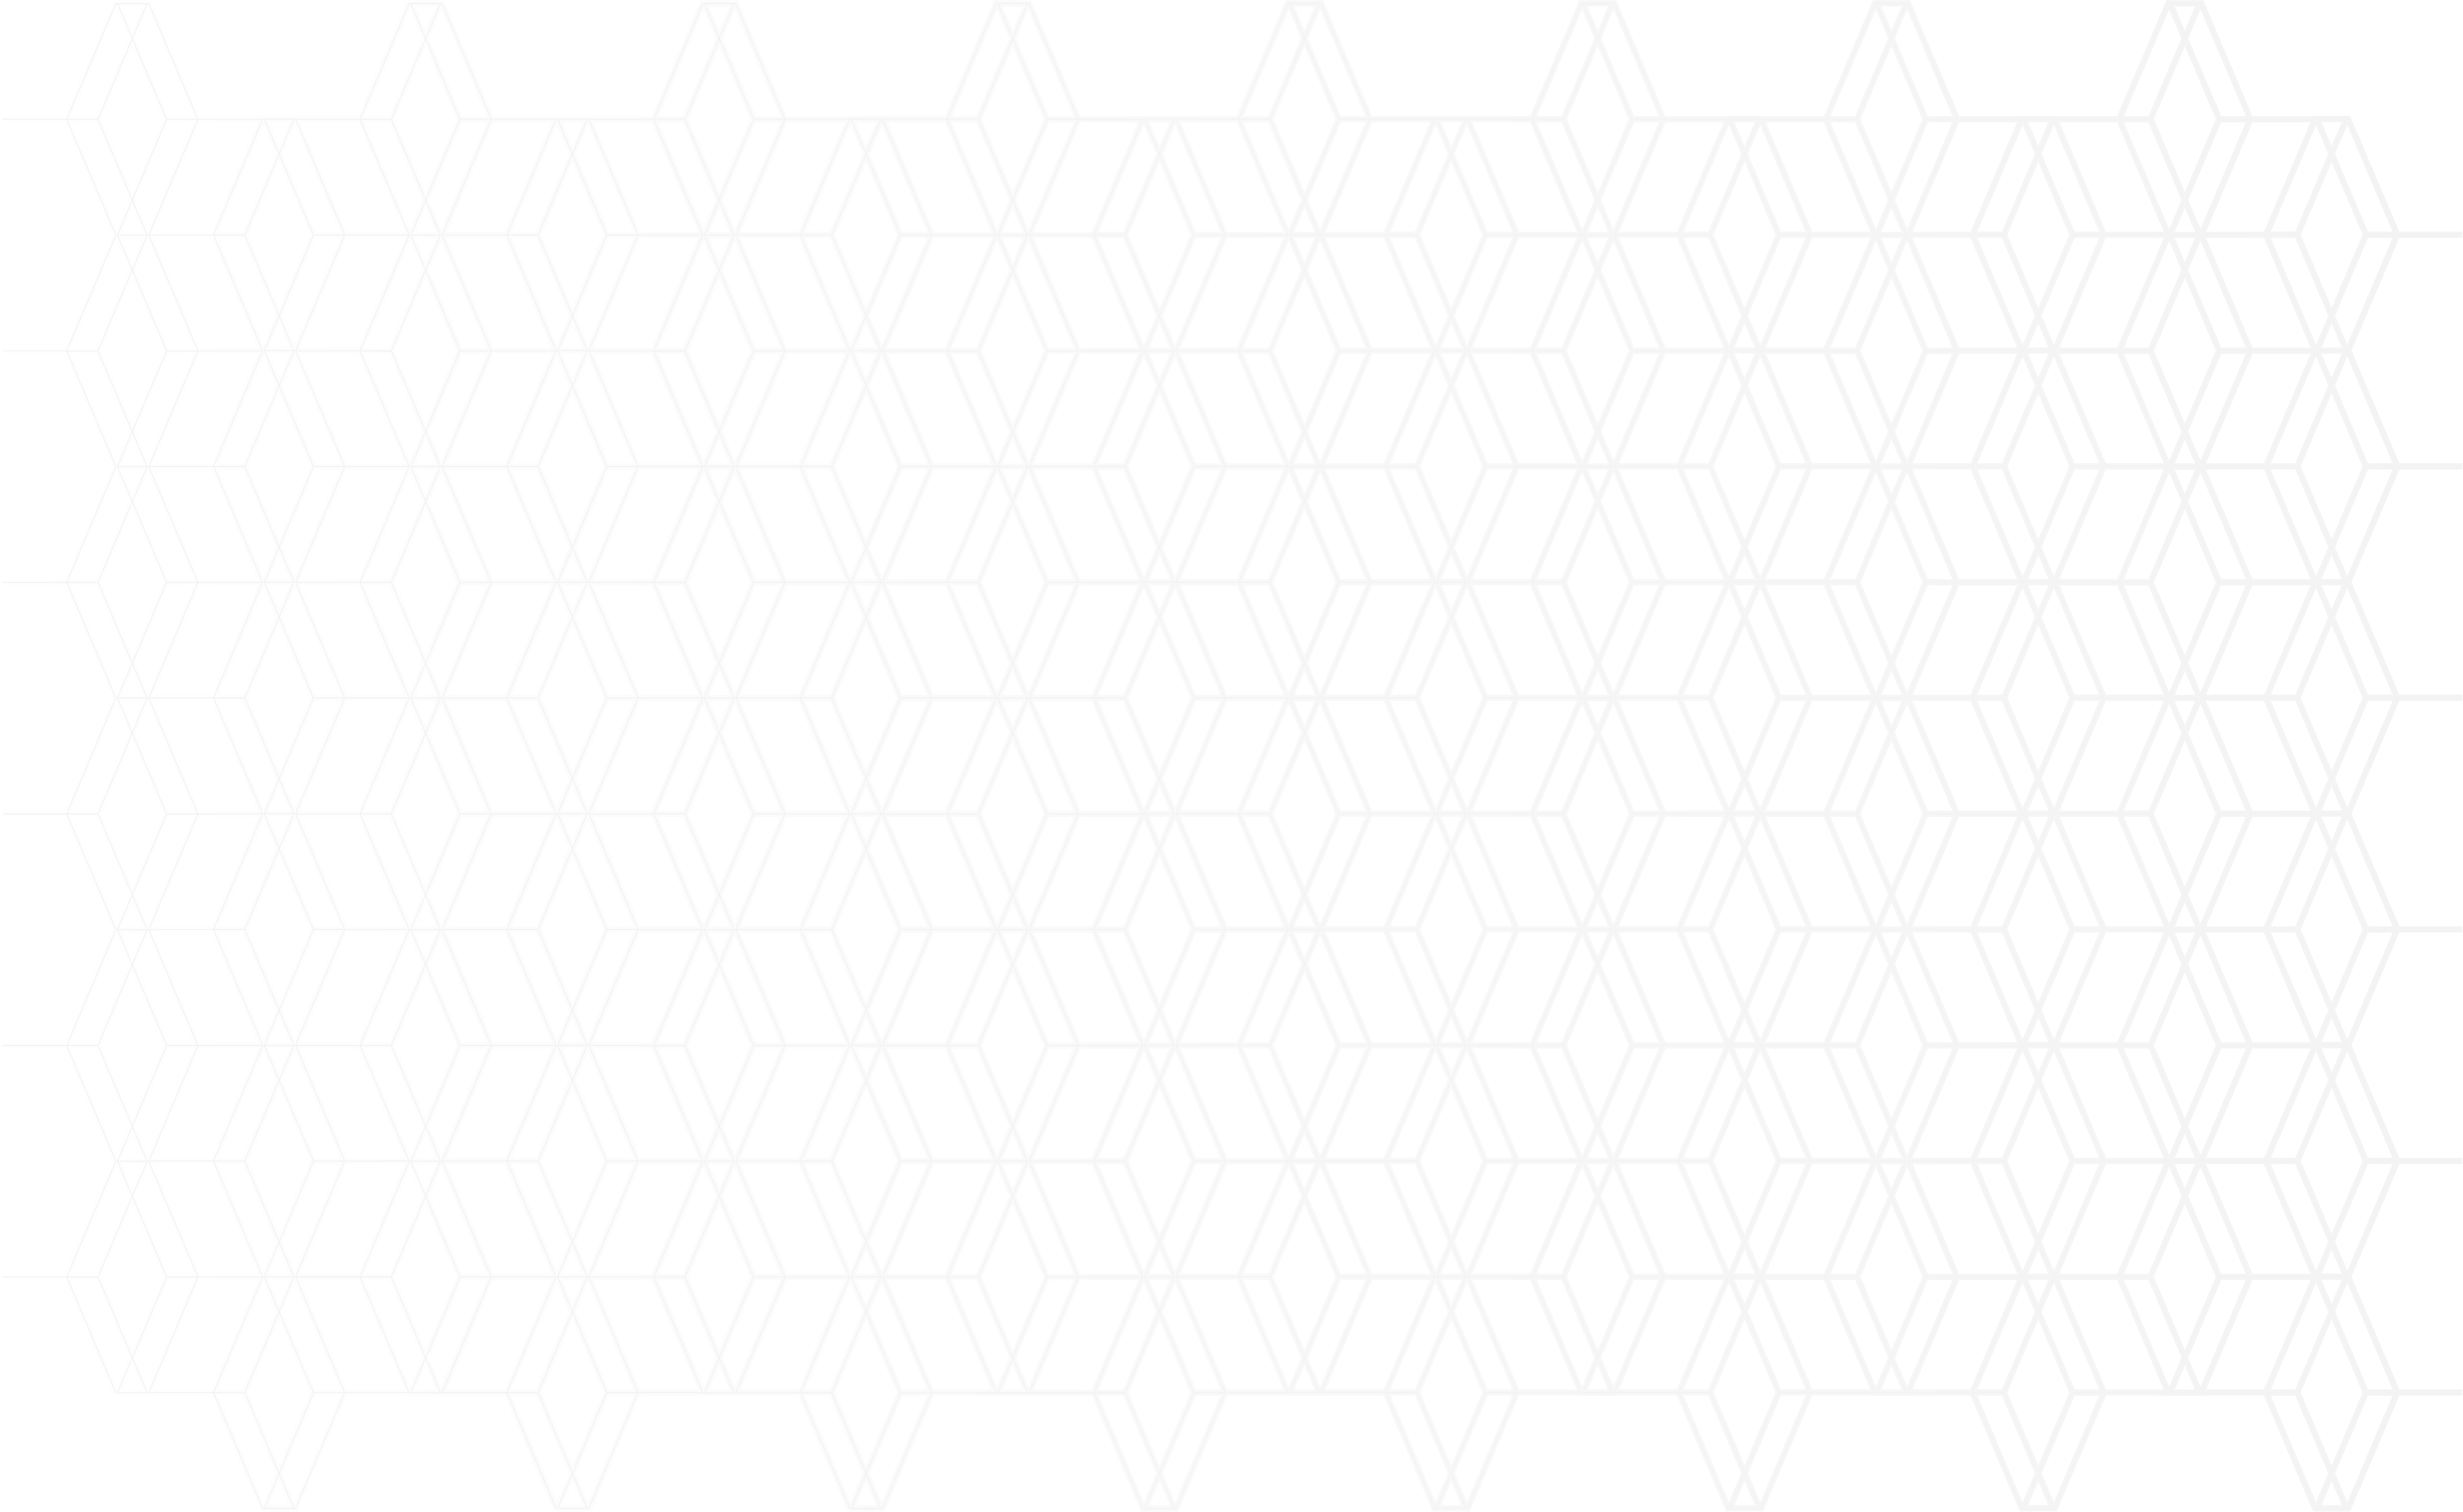
\includegraphics[width=\paperwidth]{bground.png}}
\vspace{-0.15cm}
\noindent\makebox[\linewidth]{\rule{\paperwidth}{2pt}}

\begin{multicols}{3}
\setlength{\premulticols}{1pt}
\setlength{\postmulticols}{1pt}
\setlength{\multicolsep}{1pt}
\setlength{\columnsep}{2pt}

\vfill
\section{
\includegraphics[height=\fontcharht\font`\S]{slash.png} Launching MotorCAD using PyMotorCAD}
To launch Motor-CAD instance locally and exit:
\begin{lstlisting}[language=Python]
import ansys.motorcad.core as pymotorcad
mcad = pymotorcad.MotorCAD()
mcad.load_from_file(r'path/motor_cad.mot')
# loading pre-defined template
mcad.load_template(template_name)
# saving file to working_folder
mcad.save_to_file(os.path.join(working_folder, mcad_name + ".mot"))
# existing MotorCAD
mcad.quit()
\end{lstlisting}

%\section{
\includegraphics[height=\fontcharht\font`\S]{slash.png} Loading Template}
%To load template and save file:
%\begin{lstlisting}[language=Python]
%mcad.load_template(template_name)
%mcad.save_to_file(os.path.join(working_folder, mcad_name + ".mot"))
%\end{lstlisting}

\section{
\includegraphics[height=\fontcharht\font`\S]{slash.png} Geometrical properties}
To set the motor geometry:
\begin{lstlisting}[language=Python]
mcad.set_variable("Slot_Number", 24)
mcad.set_variable("Tooth_Width", 6)
mcad.set_variable("Magnet_Thickness", 4.5)
mcad.set_variable("Pole_Number", 4)
\end{lstlisting}
To set winding patterns:
\begin{lstlisting}[language=Python]
mcad.set_variable('MagWindingType', 1)
set_variable("MagTurnsConductor",12)
\end{lstlisting}

\section{
\includegraphics[height=\fontcharht\font`\S]{slash.png} Material Assignment}
To set stater and rotor lamination materials:
\begin{lstlisting}[language=Python]
mcad.set_component_material("Stator Lam (Back Iron)", "M250-35A")
mcad.set_component_material("Rotor Lam (Back Iron)", "M250-35A")
\end{lstlisting}

\section{
\includegraphics[height=\fontcharht\font`\S]{slash.png} Building Model}
To set building commands:
\begin{lstlisting}[language=Python]
#Build options
mcad.set_variable("ModelType_MotorLAB", 1)
mcad.set_variable("SatModelPoints_MotorLAB", 0)
mcad.set_variable("LossModel_Lab", 0)
mcad.set_variable("ModelBuildSpeed_MotorLAB", 10000)
mcad.set_variable("MaxModelCurrent_MotorLAB", 480)
mcad.set_variable("BuildSatModel_MotorLAB",True)

# Setting lab context and building model
mcad.set_motorlab_context()
mcad.clear_model_build_lab()
mcad.build_model_lab()
\end{lstlisting}
\section{
\includegraphics[height=\fontcharht\font`\S]{slash.png} E-magnetic Performance Curves in LAB}
To set lab operating mode:
\begin{lstlisting}[language=Python]
mcad.set_variable("OperatingMode_Lab", 0)
# setting magnetic calculation options
mcad.set_variable("EmagneticCalcType_Lab", 0)
mcad.set_variable("SpeedMax_MotorLAB", 10000)
mcad.set_variable("Speedinc_MotorLAB", 250)
mcad.set_variable("SpeedMin_MotorLAB", 500)
mcad.set_variable("Imax_MotorLAB", 480)	
\end{lstlisting}
To calculate e-magnetic performance:
\begin{lstlisting}[language=Python]
mcad.calculate_magnetic_lab()
\end{lstlisting}

\section{
\includegraphics[height=\fontcharht\font`\S]{slash.png} Operating Point Calculation}
 To set operating point for calculations:
\begin{lstlisting}[language=Python]
mcad.set_variable("OpPointSpec_MotorLAB", 1)
mcad.set_variable("StatorCurrentDemand_Lab", 480)
mcad.set_variable("SpeedDemand_MotorLAB", 4000)
mcad.set_variable("LabThermalCoupling", 0)
mcad.set_variable("LabMagneticCoupling", 0)
\end{lstlisting}
To calculate operating point:
\begin{lstlisting}[language=Python]
mcad.calculate_operating_point_lab()
\end{lstlisting}
\section{
\includegraphics[height=\fontcharht\font`\S]{slash.png} Electromagnetic Calculations in Emag}
To perform electromagnetic calculations:
\begin{lstlisting}[language=Python]
# Set the torque calculation options.
points_per_cycle = 60 
number_cycles = 1
mcad.set_variable("TorquePointsPerCycle", points_per_cycle)
mcad.set_variable("TorqueNumberCycles", number_cycles)
# Disable all performance tests except the ones for transient torque.
mcad.set_variable("BackEMFCalculation", False)
mcad.set_variable("CoggingTorqueCalculation", False)
# Enable transient torque.
mcad.set_variable("TorqueCalculation", True)
# For running  Emag performance tests
mcad.do_magnetic_calculation ()
\end{lstlisting}


\section{
\includegraphics[height=\fontcharht\font`\S]{slash.png} Results}
\begin{lstlisting}[language=Python]
# Getting the transient torque waveform in Emag 
for n in range(points_per_cycle):
(x, y)=mcad.get_magnetic_graph_point("TorqueVW", n)
rotor_position.append(x)
torque_.append(y)
# line voltage calculation
line_voltage = mcad.get_variable("PeakLineLineVoltage")
# Retrieving lab performance curves 
data = io.loadmat(os.path.join(working_folder, mcad_name, "Lab", "MotorLAB_elecdata.mat"))
speed = data["Speed"]
shaft_torque = data["Shaft_Torque"]
shaft_power = data["Shaft_Power"]
\end{lstlisting}

\section{
\includegraphics[height=\fontcharht\font`\S]{slash.png} PyMotorCAD Scripting in MATLAB}
The Python version that MATLAB is using has the \textit{ansys.motorcad.core} package installed, PyMotorCAD is available to use in MATLAB.

To import the ansys.motorcad.core module as pymotorcad for use in scripts
\begin{lstlisting}[language=Python]
pymotorcad = py.importlib.import_module('ansys.motorcad.core')	
\end{lstlisting}

\section{
\includegraphics[height=\fontcharht\font`\S]{slash.png} Backwards Compatibility}
Old ActiveX scripts use this code to connect to Motor-CAD
\begin{lstlisting}[language=Python]
import win32com.client
mcad = win32com.client.Dispatch("MotorCAD.AppAutomation")
\end{lstlisting}
To use PyMotorCAD to connect to Motor-CAD, you replace the preceding code with this code:	
\begin{lstlisting}[language=Python]
import ansys.motorcad.core as pymotorcad
mcad = pymotorcad.MotorCADCompatibility()
\end{lstlisting}	


\subsection{References from PyMotorCad Documentation}
\begin{itemize}
\item \href{https://motorcad.docs.pyansys.com/version/stable/getting_started/index.html}{\color{blue}{Getting Started}}
\item \href{https://motorcad.docs.pyansys.com/version/stable/examples/index.html}{\color{blue}{Examples}}
\item \href{https://motorcad.docs.pyansys.com/version/stable/methods/index.html}{\color{blue}{API Reference}}
\end{itemize}
\end{multicols}

\vspace{-0.15cm}
\noindent\makebox[\linewidth]{\rule{\paperwidth}{4pt}}
\begin{center}
Getting Started with PyMotorcad 
\includegraphics[height=\fontcharht\font`\S]{slash.png} \href{https://github.com/ansys/pymotorcad}{\color{blue}{PyMotorcad on GitHub}} 
\includegraphics[height=\fontcharht\font`\S]{slash.png} Visit \code{\href{motorcad.docs.pyansys.com}}{\color{blue}{motorcad.docs.pyansys.com}}
\end{center}
\end{document}